%===================================================================
% 1º TRABALHO DE CEL115 - ELETRÔNICA ANALÓGICA II
%===================================================================
\documentclass[12pt,a4paper]{report}

\usepackage{xcolor}            % necessário para o \definecolor do template
\usepackage{template}          % template da disciplina (template.sty)
\usepackage{lmodern}           % fontes vetoriais na codificação T1 do template
\usepackage{icomma}            % vírgula decimal em modo matemático
\usepackage{amssymb}
\usepackage{array}
\usepackage{enumitem}
% Os circuitos (circuitikz) e os gráficos (pgfplots) estão pré-compilados em
% PDF na pasta figuras/, o que reduz o tempo de compilação no Overleaf. Os
% gráficos saem de figuras/src/graficos.tex, com os dados exportados das
% simulações do LTspice (figuras/src/*.dat).

\setlist[enumerate]{leftmargin=*, itemsep=3pt}
\makeatletter
\renewcommand{\thefigure}{\thechapter.\@arabic\c@figure}
\renewcommand{\thetable}{\thechapter.\@arabic\c@table}
\renewcommand{\theequation}{\thechapter.\@arabic\c@equation}
\makeatother
\setlist[itemize]{itemsep=2pt}

% Figuras flutuantes: podem ocupar quase toda a página, no topo ou no pé,
% sem deixar buracos.
\renewcommand{\topfraction}{0.9}
\renewcommand{\bottomfraction}{0.8}
\renewcommand{\textfraction}{0.07}
\renewcommand{\floatpagefraction}{0.75}
\setcounter{topnumber}{2}
\setcounter{bottomnumber}{2}
\setcounter{totalnumber}{4}

% Respiro vertical nas tabelas
\renewcommand{\arraystretch}{1.3}

% Sem linha isolada no topo ou no pé da página
\widowpenalty=10000
\clubpenalty=10000
\displaywidowpenalty=10000

% ---------- Unidades ----------
\newcommand{\un}[1]{\,\mathrm{#1}}
\newcommand{\kohm}{\un{k\Omega}}
\newcommand{\Om}{\un{\Omega}}
\newcommand{\uA}{\,\text{\textmu A}}
\newcommand{\uF}{\,\text{\textmu F}}
\newcommand{\uAV}{\,\text{\textmu A/V}}
\newcommand{\mAV}{\un{mA/V}}
\newcommand{\resposta}{\par\smallskip\noindent\textbf{Resposta.}\ }

%===================================================================
% DADOS DA CAPA
%===================================================================
\competicao{Faculdade de Engenharia}
\disciplina{1º Trabalho\\[0.3cm] CEL115 -- Eletrônica Analógica II}
\alunos{Angelo V. A. V. da Silva, matrícula 202169001A\\[0.2cm] Chrysthofer A. A. Afonso, matrícula 202269001A}
\logocapa{figuras/logo_ufjf.png}
\logocabecalho{figuras/LogoUFJF.jpg}

%===================================================================
\begin{document}
\renewcommand{\today}{12 de outubro de 2026}

% A capa e o sumário recebem o número de página 1; a capa fica sem âncora
% para o hyperref não duplicar o destino page.1.
\hypersetup{pageanchor=false}
\maketitlepage
\hypersetup{pageanchor=true}
% Definida depois da capa: o nome da universidade já está no logotipo da
% capa, e a sigla cabe na célula do rodapé.
\instituicao{UFJF}
\pagestyle{IHA-fancy-plain}

\tableofcontents
\listoffigures

%===================================================================
\chapter*{Introdução}
\addcontentsline{toc}{chapter}{Introdução}
\markboth{Introdução}{}
%===================================================================

Cada questão do enunciado ocupa um capítulo, com uma seção por item. O Capítulo~\ref{cap:conclusao} reúne as respostas e o erro de cada uma em relação à simulação. Convenções usadas em todo o relatório:
\begin{itemize}
    \item Letra maiúscula com índice maiúsculo ($I_D$, $V_{GS}$) indica polarização; letra minúscula ($i_d$, $v_{gs}$), sinal. Na polarização os capacitores são abertos. Para o sinal, as fontes c.c. são terra; nas médias frequências os capacitores de acoplamento são curtos e as capacitâncias internas do transistor, abertas.
    \item MOSFET na saturação: $I_D = \tfrac12 k_n'\tfrac{W}{L}V_{OV}^2(1+\lambda V_{DS})$, com $V_{OV} = V_{GS}-V_{tn}$, exigindo $V_{GS} > V_{tn}$ e $V_{DS}\geq V_{OV}$. Como é usual, o fator $(1+\lambda V_{DS})$ é desprezado na polarização, e $\lambda$ entra no sinal pela resistência $r_o = 1/(\lambda I_D)$. A transcondutância é $g_m = 2I_D/V_{OV}$.
    \item Transistor bipolar no modo ativo: $I_C = \beta I_B = \alpha I_E$, com $\alpha = \beta/(\beta+1)$, $g_m = I_C/V_T$, $r_e = V_T/I_E$ e $V_T = 25$~mV.
    \item $R_1\parallel R_2 = R_1R_2/(R_1+R_2)$; $|A|_{dB} = 20\log_{10}|A|$. As frequências de corte $f_L$ (inferior) e $f_H$ (superior) são aquelas em que o ganho cai 3~dB abaixo do de médias frequências.
    \item As contas foram feitas sem arredondar e os valores aparecem com três ou quatro algarismos significativos; refazê-las com os valores arredondados pode mudar a última casa.
    \item As simulações são as \textit{netlists} do LTspice da pasta \texttt{simulacoes/}: \texttt{\_cc} calcula a polarização (\texttt{.op}), \texttt{\_transiente} simula no tempo (\texttt{.tran}) e \texttt{\_frequencia} dá a resposta em frequência (\texttt{.ac}). Os valores citados vêm de comandos \texttt{.meas}, gravados no arquivo \texttt{.log}, e os gráficos foram traçados por nós com os dados exportados dessas simulações. O erro percentual é a diferença entre o valor simulado e o calculado, dividida pelo calculado.
\end{itemize}

Os arquivos de simulação estão em
\begin{center}
\small\url{https://github.com/Chrysthofer/TRAB-I-ELE-ANALOG-II-ENTREGA/tree/main/simulacoes}
\end{center}

%===================================================================
\chapter{Questão 1}
%===================================================================

A Questão 1 trata do amplificador de dois estágios com MOSFETs da Figura~\ref{fig:q1-circuito}. Os dois transistores são idênticos, com
\begin{equation*}
k_n'\frac{W}{L} = 8\un{mA/V^2}, \qquad V_{tn} = 2\un{V}, \qquad \lambda = 0{,}01\un{V^{-1}}.
\end{equation*}

\begin{figure}[htbp]
\centering
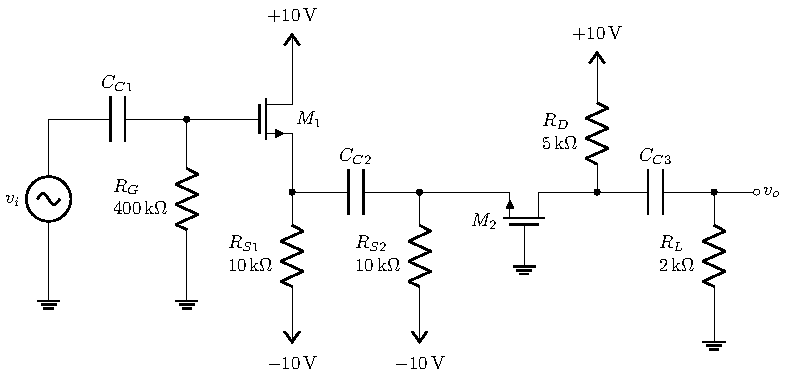
\includegraphics{figuras/fig_q1_circuito}
\caption{Amplificador de dois estágios com MOSFETs da Questão 1.}
\label{fig:q1-circuito}
\end{figure}

M1 recebe o sinal na porta e o entrega na fonte, com o dreno em $+10$~V: é um \textbf{dreno-comum} (seguidor de fonte), de alta resistência de entrada e baixa resistência de saída. M2 recebe o sinal na fonte, via $C_{C2}$, e o entrega no dreno, com a porta aterrada: é um \textbf{porta-comum}, que fornece o ganho de tensão.

%-------------------------------------------------------------------
\section{Item (a): \texorpdfstring{$I_{D1}$, $I_{D2}$, $V_{DS1}$ e $V_{DS2}$}{ID1, ID2, VDS1 e VDS2}}
%-------------------------------------------------------------------

Com os capacitores abertos, os dois transistores ficam separados (Figura~\ref{fig:q1-cc}). Como a corrente de porta é nula, não há queda em $R_G$ e $V_{G1} = 0$; a porta de M2 está aterrada, então $V_{G2} = 0$. Nos dois transistores a fonte vai a $-10$~V por $10\kohm$: as malhas porta-fonte são iguais e as correntes também. $R_D$ só fixa a tensão de dreno de M2.

\begin{figure}[htbp]
\centering
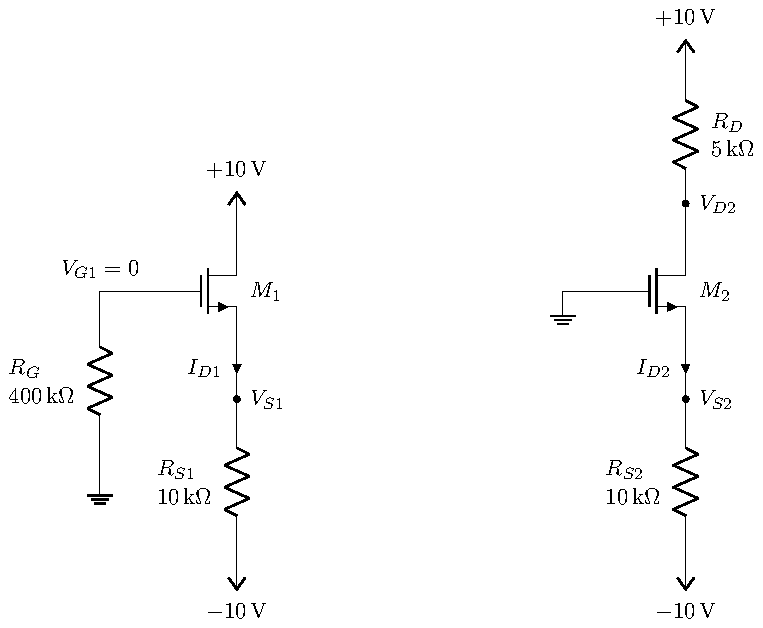
\includegraphics{figuras/fig_q1_cc}
\caption{Circuito equivalente c.c. da Questão 1, com os capacitores abertos.}
\label{fig:q1-cc}
\end{figure}

A corrente que desce por $R_S$ é a de dreno. Com $V_{GS} = 2 + V_{OV}$, corrente em mA e resistência em k$\Omega$:
\begin{gather*}
I_D = \frac{10 - V_{GS}}{10} = \frac12\cdot8\cdot V_{OV}^2
\;\Rightarrow\; 8 - V_{OV} = 40\,V_{OV}^2,\\[2pt]
V_{OV} = \frac{-1\pm\sqrt{1+4\cdot40\cdot8}}{80} = \frac{-1\pm35{,}791}{80}.
\end{gather*}
A raiz negativa, $-0{,}4599$~V, daria $V_{GS} < V_{tn}$, sem canal, e é descartada. Fica $V_{OV} = 0{,}4349$~V, $V_{GS} = 2{,}435$~V e
\begin{align*}
I_{D1} = I_{D2} &= 4\times0{,}4349^2 = 0{,}7565\un{mA},\\[4pt]
V_{DS1} &= 10 - (-2{,}435) = 12{,}43\un{V},\\[4pt]
V_{D2} &= 10 - 5\times0{,}7565 = 6{,}217\un{V},\\[4pt]
V_{DS2} &= 6{,}217 - (-2{,}435) = 8{,}652\un{V}.
\end{align*}

A Tabela~\ref{tab:q1-cc} verifica as duas condições de saturação.

\begin{table}[H]
\centering
\caption{Polarização dos transistores da Questão 1 e verificação da saturação.}
\label{tab:q1-cc}
\begin{tabular}{lcccccc}
\toprule
 & $I_D$ (mA) & $V_{GS}$ (V) & $V_{OV}$ (V) & $V_{DS}$ (V) & $V_{GS}>V_{tn}$? & $V_{DS}\geq V_{OV}$? \\
\midrule
M1 & 0,7565 & 2,435 & 0,435 & 12,43 & Sim & Sim (folga de 12~V) \\
M2 & 0,7565 & 2,435 & 0,435 & 8,652 & Sim & Sim (folga de 8,2~V) \\
\bottomrule
\end{tabular}
\end{table}

\resposta $I_{D1} = I_{D2} = 0{,}757$~mA, $V_{DS1} = 12{,}43$~V e $V_{DS2} = 8{,}65$~V. Os dois transistores estão saturados com folga: o dreno de M2 pode descer cerca de 8~V antes de entrar na região de triodo, então estão bem polarizados para amplificar.

%-------------------------------------------------------------------
\section{Item (b): ganho de tensão em médias frequências}
%-------------------------------------------------------------------

Os dois transistores têm a mesma corrente e a mesma $V_{OV}$, logo os mesmos parâmetros de sinal:
\begin{gather*}
g_m = \frac{2\times0{,}7565\un{mA}}{0{,}4349\un{V}} = 3{,}479\mAV,\qquad \frac{1}{g_m} = 287{,}4\Om,\\[2pt]
r_o = \frac{1}{0{,}01\times0{,}7565\un{mA}} = 132{,}2\kohm,\qquad g_mr_o = 459{,}9.
\end{gather*}
Para o sinal, o dreno de M1 fica em terra, $R_{S1}$, $R_{S2}$ e $R_D$ vão para o terra, a porta de M1 recebe $v_i$ diretamente e $R_L$ fica em paralelo com $R_D$. Os transistores são representados pelo modelo T, conveniente quando o sinal entra ou sai pela fonte \cite{notas}.

\subsection{Modelo genérico e associação}

Cada estágio vira um amplificador de tensão genérico (Figura~\ref{fig:q1-generico}) \cite{sedra}, descrito pela resistência de entrada $R_{\mathrm{in}}$, pelo ganho em circuito aberto $A_{vo}$ e pela resistência de saída $R_o$, esta calculada com a entrada do estágio zerada. Cada bloco inclui seus resistores: o estágio 1 é $R_G$, M1 e $R_{S1}$; o estágio 2, $R_{S2}$, M2 e $R_D$. O ganho total é
\begin{equation}
\frac{v_o}{v_i} = \frac{v_{i1}}{v_i}\cdot A_{vo1}\cdot\frac{R_{\mathrm{in}2}}{R_{\mathrm{in}2}+R_{o1}}\cdot A_{vo2}\cdot\frac{R_L}{R_L+R_{o2}},
\label{eq:q1-assoc}
\end{equation}
com $v_{i1}/v_i = 1$, porque $v_i$ é uma fonte ideal ligada direto à porta. Com $r_o$, o porta-comum deixa de ser unilateral: $r_o$ liga a fonte ao dreno de M2, e $R_{\mathrm{in}2}$ passa a depender da carga. Calculando $R_{\mathrm{in}2}$ com $R_L$ ligado e $R_{o2}$ com $v_{i2} = 0$, a expressão~\eqref{eq:q1-assoc} é exata.

\begin{figure}[htbp]
\centering
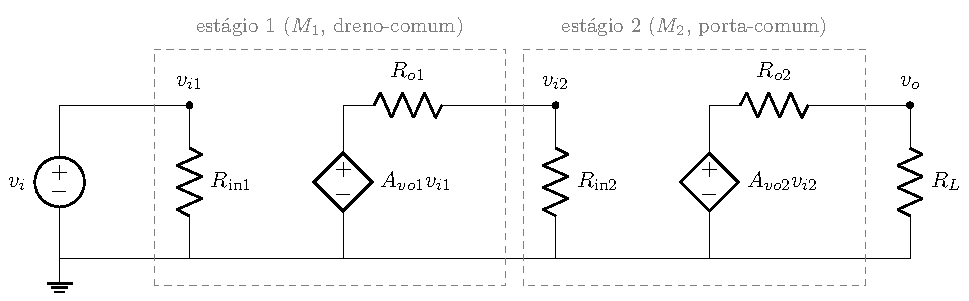
\includegraphics{figuras/fig_c_q1_generico}
\caption[Os dois estágios da Questão 1 no modelo genérico de amplificador de tensão.]{Os dois estágios da Questão 1 no modelo genérico de amplificador de tensão; $v_{i1}$, $v_{i2}$ e $v_o$ são tensões em relação ao terra.}
\label{fig:q1-generico}
\end{figure}

\subsection{Estágio 1: dreno-comum}

Na Figura~\ref{fig:q1-est1}, o dreno $D_1$ está em terra; por isso $r_o$ fica em paralelo com $R_{S1}$: $R_{S1}' = R_{S1}\parallel r_o = 9{,}297\kohm$.

\begin{figure}[htbp]
\centering
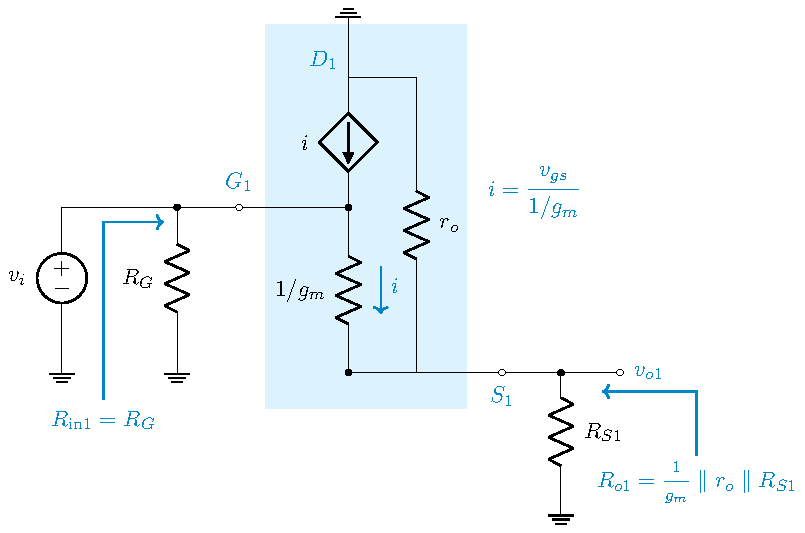
\includegraphics{figuras/fig_q1_est1_T}
\caption{Estágio 1 da Questão 1 (dreno-comum) com M1 no modelo T, na região sombreada.}
\label{fig:q1-est1}
\end{figure}

A corrente que a fonte controlada injeta na porta é a mesma que $1/g_m$ retira, então a porta não puxa corrente e só $R_G$ aparece. Na saída aberta, $v_s = g_m(v_{i1}-v_s)R_{S1}'$. Com a porta em terra, olhando da fonte há três caminhos para o terra: $1/g_m$, $r_o$ e $R_{S1}$.
\begin{gather*}
\boxed{R_{\mathrm{in}1} = R_G = 400\kohm}\\[6pt]
\boxed{A_{vo1} = \frac{g_mR_{S1}'}{1+g_mR_{S1}'} = 0{,}9700}\\[6pt]
\boxed{R_{o1} = \frac{1}{g_m}\parallel r_o\parallel R_{S1} = 278{,}8\Om}
\end{gather*}

\subsection{Estágio 2: porta-comum}

Na Figura~\ref{fig:q1-est2}, a porta $G_2$ está em terra; com $v_{i2}$ na fonte de M2, a corrente em $1/g_m$ é $i = -g_mv_{i2}$, e ela percorre a fonte controlada. A lei das correntes no dreno, sem $R_L$, dá o ganho em circuito aberto:
\begin{gather*}
\frac{v_d}{R_D} + \frac{v_d - v_{i2}}{r_o} - g_mv_{i2} = 0
\;\Rightarrow\;
A_{vo2} = \frac{v_d}{v_{i2}} = \left(g_m+\frac{1}{r_o}\right)(R_D\parallel r_o),\\[2pt]
\boxed{A_{vo2} = 3{,}487\mAV\times4{,}818\kohm = 16{,}80}
\end{gather*}
Com $v_{i2} = 0$, as duas pontas de $1/g_m$ ficam em terra e $i = 0$; do dreno se vê só $R_D$ em paralelo com $r_o$:
\begin{equation*}
\boxed{R_{o2} = R_D\parallel r_o = 4{,}818\kohm}
\end{equation*}

\begin{figure}[htbp]
\centering
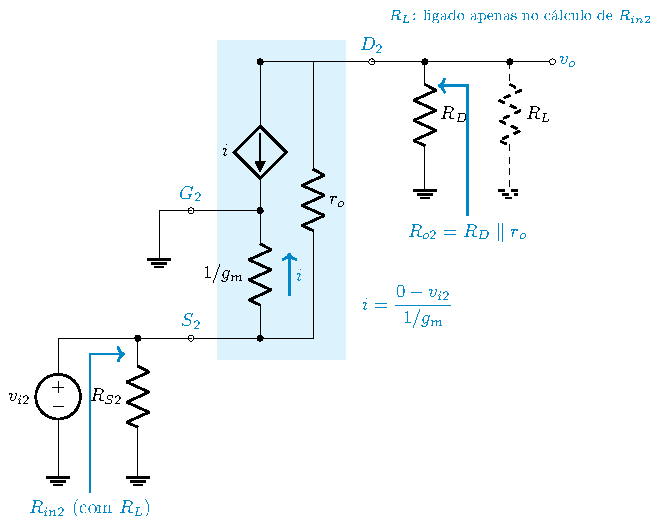
\includegraphics{figuras/fig_q1_est2_T}
\caption{Estágio 2 da Questão 1 (porta-comum) com M2 no modelo T, na região sombreada.}
\label{fig:q1-est2}
\end{figure}

Para $R_{\mathrm{in}2}$, aplica-se $v_x$ na fonte de M2 com a carga real no dreno, $R_L' = R_D\parallel R_L = 1{,}429\kohm$. A mesma lei das correntes dá $v_d = v_x(g_m + 1/r_o)(R_L'\parallel r_o)$, e a corrente que entra no transistor, $i_t = g_mv_x + (v_x - v_d)/r_o$, resulta em
\begin{gather*}
R_{\mathrm{in},s} = \frac{v_x}{i_t} = \frac{r_o + R_L'}{1 + g_mr_o} = \frac{133{,}6\kohm}{460{,}9} = 289{,}9\Om,\\[6pt]
\boxed{R_{\mathrm{in}2} = R_{S2}\parallel R_{\mathrm{in},s} = 281{,}7\Om}
\end{gather*}

\subsection{Associação dos estágios e efeito de \texorpdfstring{$r_o$}{ro}}

Levando os parâmetros à expressão~\eqref{eq:q1-assoc}:
\begin{align*}
\frac{v_o}{v_i} &= 1\times0{,}9700\times\frac{281{,}7}{281{,}7+278{,}8}\times16{,}80\times\frac{2}{2+4{,}818}\\[4pt]
&= 0{,}9700\times0{,}5026\times16{,}80\times0{,}2934 = 2{,}40.
\end{align*}
Metade do sinal se perde entre os estágios, porque a entrada do porta-comum (282~$\Omega$) é tão baixa quanto a saída do seguidor (279~$\Omega$), e na saída só 29\% de $A_{vo2}v_{i2}$ chega a $R_L$. Resolver o circuito de sinal inteiro por análise nodal, sem separar os estágios, dá o mesmo 2,402.

A Tabela~\ref{tab:q1-ro} mostra o efeito de $r_o$ nos dois transistores. Ele reduz o ganho em 0,5\%, porque $r_o = 132\kohm$ é muito maior que as resistências em paralelo com ele; o efeito maior está em $A_{vo2}$, em parte compensado pela queda de $R_{o2}$.

\begin{table}[H]
\centering
\caption{Parâmetros dos estágios da Questão 1 com e sem $r_o$.}
\label{tab:q1-ro}
\begin{tabular}{lcccccc}
\toprule
 & $A_{vo1}$ & $R_{o1}$ ($\Omega$) & $R_{\mathrm{in}2}$ ($\Omega$) & $A_{vo2}$ & $R_{o2}$ (k$\Omega$) & $v_o/v_i$ \\
\midrule
Com $r_o$ & 0,9700 & 278,8 & 281,7 & 16,80 & 4,818 & 2,402 \\
Sem $r_o$ & 0,9721 & 279,4 & 279,4 & 17,40 & 5,000 & 2,416 \\
\bottomrule
\end{tabular}
\end{table}

\resposta $v_o/v_i = +2{,}40$~V/V, ou 7,6~dB, com a saída em fase com a entrada.

%-------------------------------------------------------------------
\section{Item (c): projeto dos capacitores de acoplamento}
%-------------------------------------------------------------------

O item pede $f_L = 100$~Hz. Em baixas frequências cada capacitor de acoplamento forma, com a resistência $R_i$ que ele enxerga, um passa-altas de corte $f_{Pi} = 1/(2\pi R_iC_i)$. O método das constantes de tempo de curto-circuito estima $f_L\approx\sum f_{Pi}$, com $R_i$ calculada com $v_i = 0$ e os outros capacitores em curto. A Tabela~\ref{tab:q1-cap} reúne as resistências e o projeto.

\begin{table}[H]
\centering
\caption{Resistência vista por cada capacitor de acoplamento da Questão 1 e capacitores do método.}
\label{tab:q1-cap}
\begin{tabular}{lcccc}
\toprule
Capacitor & Resistência vista & Valor & $f_{Pi}$ & $C_i = 1/(2\pi R_if_{Pi})$ \\
\midrule
$C_{C1}$ & $R_G$ & 400~k$\Omega$ & 10~Hz & 39,79~nF \\
$C_{C2}$ & $R_{o1} + R_{\mathrm{in}2}$ & 560,5~$\Omega$ & 80~Hz & 3,549~\textmu F \\
$C_{C3}$ & $(R_D\parallel R_{d2}) + R_L$ & 6,905~k$\Omega$ & 10~Hz & 2,305~\textmu F \\
\bottomrule
\end{tabular}
\end{table}

$C_{C1}$ vê só $R_G$, porque a porta não puxa corrente e a fonte zerada é um curto. $C_{C2}$ vê a saída do seguidor, $R_{o1}$, em série com a entrada do porta-comum, $R_{\mathrm{in}2}$, calculada com $R_L$ porque $C_{C3}$ está em curto. $C_{C3}$ vê $R_L$ em série com $R_D$ em paralelo com a resistência olhando para o dreno de M2, cuja fonte enxerga $R_f = R_{S2}\parallel R_{o1} = 271{,}2\Om$:
\begin{equation*}
R_{d2} = r_o + (1+g_mr_o)R_f = 132{,}2\kohm + 460{,}9\times271{,}2\Om = 257{,}2\kohm.
\end{equation*}

As frequências precisam somar 100~Hz. O capacitor que vê a menor resistência, $C_{C2}$, recebe 80\% de $f_L$, para não ficar enorme, e os outros dois, 10\% cada. Arredondando, $C_{C1} = 39{,}8$~nF, $C_{C2} = 3{,}55$~\textmu F e $C_{C3} = 2{,}31$~\textmu F.

A soma das $f_{Pi}$ só acerta $f_L$ quando um capacitor domina. Tratando os três filtros como independentes, o ganho relativo em $f$ é o produto dos fatores $f/\sqrt{f^2+f_{Pi}^2}$, que chega a $1/\sqrt2$ em $f_L\approx82{,}4$~Hz, abaixo dos 100~Hz pretendidos. Por isso o item (d) ajusta os capacitores a partir da simulação.

\resposta Pelo método, $C_{C1} = 39{,}8$~nF, $C_{C2} = 3{,}55$~\textmu F e $C_{C3} = 2{,}31$~\textmu F. Para $f_L = 100$~Hz, com o ajuste do item (d): $C_{C1} = 34{,}4$~nF, $C_{C2} = 3{,}07$~\textmu F e $C_{C3} = 2{,}00$~\textmu F.

%-------------------------------------------------------------------
\section{Item (d): simulações e comparação}
%-------------------------------------------------------------------

Os arquivos são \texttt{q1\_cc.cir}, \texttt{q1\_transiente.cir} e \texttt{q1\_frequencia.cir}; o último simula os dois conjuntos de capacitores. O MOSFET é o nível 1 do LTspice, com $\texttt{KP} = 8\un{mA/V^2}$ e $W = L$, $\texttt{VTO} = 2$~V e $\texttt{LAMBDA} = 0{,}01$/V. Esse modelo não tem capacitâncias internas, então a simulação não tem $f_H$. O transiente usa uma senoide de 10~mV de pico em 10~kHz, no meio da faixa de passagem. A Tabela~\ref{tab:q1-sim} compara os resultados, e as Figuras~\ref{fig:q1-sim-tran} e~\ref{fig:q1-sim-freq} mostram as curvas.

\begin{table}[H]
\centering
\caption{Questão 1: valores calculados nos itens (a) a (c) e simulados.}
\label{tab:q1-sim}
\begin{tabular}{lccc}
\toprule
Grandeza & Calculado & Simulado & Erro \\
\midrule
$I_{D1}$ & 0,7565~mA & 0,7589~mA & $+0{,}32\%$ \\
$I_{D2}$ & 0,7565~mA & 0,7582~mA & $+0{,}23\%$ \\
$V_{DS1}$ & 12,43~V & 12,41~V & $-0{,}19\%$ \\
$V_{DS2}$ & 8,652~V & 8,627~V & $-0{,}30\%$ \\
$v_o/v_i$, transiente em 10~kHz & 2,402 & 2,536 & $+5{,}57\%$ \\
$v_o/v_i$, resposta em frequência em 10~kHz & 2,402 & 2,533 & $+5{,}45\%$ \\
$f_L$, capacitores do método & 82,4~Hz & 86,47~Hz & $+4{,}92\%$ \\
$f_L$, capacitores ajustados & 100~Hz (projeto) & 99,98~Hz & $-0{,}02\%$ \\
\bottomrule
\end{tabular}
\end{table}

\begin{figure}[htbp]
\centering
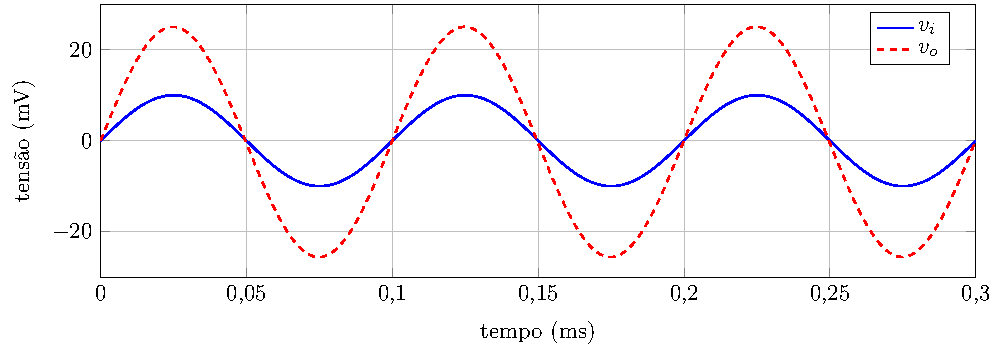
\includegraphics{figuras/fig_c_q1_transiente}
\caption[Questão 1: entrada e saída simuladas no transiente.]{Questão 1: entrada e saída simuladas no transiente, com 10~mV de pico em 10~kHz. A saída está em fase com a entrada.}
\label{fig:q1-sim-tran}
\end{figure}

\begin{figure}[htbp]
\centering
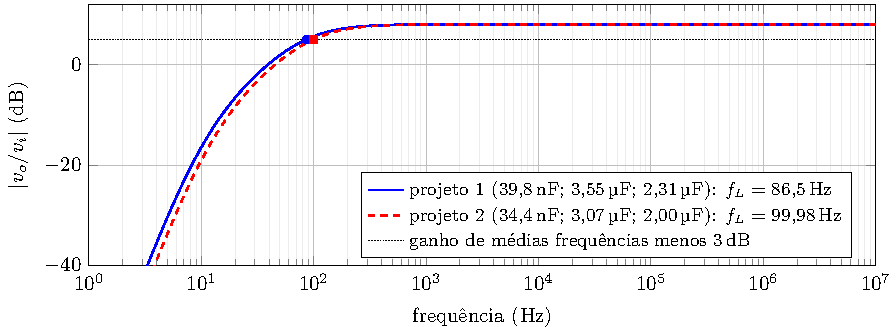
\includegraphics{figuras/fig_c_q1_frequencia}
\caption[Questão 1: módulo do ganho simulado em função da frequência.]{Questão 1: módulo do ganho simulado em função da frequência, com os capacitores do método (39,8~nF; 3,55~\textmu F; 2,31~\textmu F) e com os ajustados (34,4~nF; 3,07~\textmu F; 2,00~\textmu F). Os marcadores indicam $f_L$, onde cada curva cruza a linha 3~dB abaixo do ganho de médias frequências.}
\label{fig:q1-sim-freq}
\end{figure}

Para os capacitores do método, o valor calculado de $f_L$ é a estimativa de 82,4~Hz do item (c), e não os 100~Hz da soma das frequências. A polarização simulada difere da calculada em menos de 0,4\%, e o ganho e a fase em 10~kHz ($+0{,}6^\circ$ e $+0{,}7^\circ$ para os dois conjuntos de capacitores) confirmam a saída em fase. O ganho simulado fica 5\% acima do calculado porque o LTspice mantém o fator $(1+\lambda V_{DS})$ na polarização, que vale 1,124 em M1 e 1,086 em M2. A mesma corrente passa a ser obtida com $V_{OV}$ menor, 0,411~V e 0,418~V em vez de 0,435~V, e $g_m = 2I_D/V_{OV}$ sobe para 3,69~mA/V e 3,63~mA/V; o simulador também usa $r_o = (1+\lambda V_{DS})/(\lambda I_D)$, 148~k$\Omega$ e 143~k$\Omega$. Refazendo o item (b) com esses valores, obtém-se 2,533, o valor simulado. Com o mesmo $g_m$, a resistência vista por $C_{C2}$ cai de 560,5~$\Omega$ para 533,3~$\Omega$, a frequência de $C_{C2}$ sobe de 80,0~Hz para 84,1~Hz, e a conta do item (c) passa a dar 86,4~Hz, perto dos 86,47~Hz simulados.

Para chegar a 100~Hz, os três capacitores são multiplicados pelo mesmo fator $k$: como todas as $f_{Pi}$ são inversamente proporcionais às capacitâncias, a curva se desloca em frequência e $f_L$ fica dividida por $k$. Com $k = 86{,}47/100 = 0{,}865$, obtêm-se $C_{C1} = 34{,}4$~nF, $C_{C2} = 3{,}07$~\textmu F e $C_{C3} = 2{,}00$~\textmu F, e a simulação dá $f_L = 99{,}98$~Hz.

%===================================================================
\chapter{Questão 2}
%===================================================================

A Questão 2 trata do amplificador com transistor bipolar da Figura~\ref{fig:q2-circuito}, com
\begin{equation*}
\beta = 100, \qquad V_{EB} = 0{,}7\un{V}, \qquad V_A = \infty, \qquad C_\pi = 10\un{pF}, \qquad C_\mu = 1\un{pF}.
\end{equation*}

\begin{figure}[htbp]
\centering
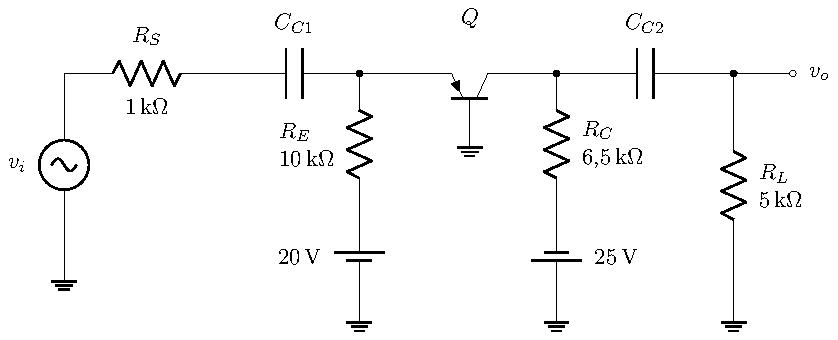
\includegraphics{figuras/fig_q2_circuito}
\caption[Amplificador com transistor PNP da Questão 2.]{Amplificador com transistor PNP da Questão 2; o traço longo de cada bateria indica o terminal positivo.}
\label{fig:q2-circuito}
\end{figure}

O transistor é PNP, a base está em terra, o sinal entra pelo emissor e sai pelo coletor: é um \textbf{base-comum}. A bateria de 20~V tem o polo positivo para cima, então $R_E$ vai a $+20$~V; a de 25~V tem o polo negativo para cima, então $R_C$ vai a $-25$~V. Adota-se $V_T = 25$~mV e resistência de base nula.

%-------------------------------------------------------------------
\section{Item (a): ganho de tensão em médias frequências}
%-------------------------------------------------------------------

\subsection{Polarização}

Com os capacitores abertos, $v_i$ e $R_L$ ficam desligados (Figura~\ref{fig:q2-cc}). No PNP a corrente entra pelo emissor e sai pelo coletor e pela base. A Tabela~\ref{tab:q2-pol} resume o ponto de operação.

\begin{figure}[htbp]
\centering
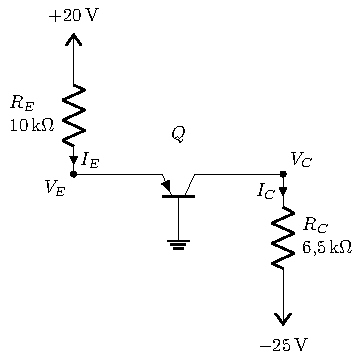
\includegraphics{figuras/fig_q2_cc}
\caption{Circuito equivalente c.c. da Questão 2.}
\label{fig:q2-cc}
\end{figure}

\begin{enumerate}
    \item A base está em 0~V e, no PNP ativo, o emissor fica 0,7~V acima: $V_E = 0{,}7$~V.
    \item A corrente de emissor desce de $+20$~V por $R_E$: $I_E = (20 - 0{,}7)/10\kohm = 1{,}930$~mA.
    \item $I_B = I_E/(\beta+1) = 19{,}11$~\textmu A e $I_C = \beta I_B = 1{,}911$~mA, que desce por $R_C$ até $-25$~V.
    \item $V_C = -25 + 6{,}5\times1{,}911 = -12{,}58$~V. Como $V_C < V_B = 0$, a junção base-coletor está reversa e o transistor está no modo ativo, com $V_{EC} = 13{,}28$~V.
\end{enumerate}

\begin{table}[H]
\centering
\caption{Ponto de operação do transistor da Questão 2.}
\label{tab:q2-pol}
\begin{tabular}{lccccc}
\toprule
$V_E$ & $I_E$ & $I_B$ & $I_C$ & $V_C$ & $V_{EC}$ \\
\midrule
0,7~V & 1,930~mA & 19,11~\textmu A & 1,911~mA & $-12{,}58$~V & 13,28~V \\
\bottomrule
\end{tabular}
\end{table}

\subsection{Ganho}

Os parâmetros de sinal são $g_m = I_C/V_T = 1{,}911\un{mA}/25\un{mV} = 76{,}44\mAV$ e $r_e = V_T/I_E = 12{,}95\Om$, com $\alpha/r_e = g_m$. Nas médias frequências $C_{C1}$ e $C_{C2}$ são curtos, $C_\pi$ e $C_\mu$ são abertos e as baterias são terra: $R_E$ vai do emissor ao terra e $R_C$ e $R_L$ ficam em paralelo no coletor. Como o sinal entra pelo emissor, usa-se o modelo T (Figura~\ref{fig:q2-T}), desenhado com os sentidos de corrente do PNP, o que deixa as expressões sem sinais negativos. Com $V_A = \infty$, nada liga o emissor ao coletor além da fonte controlada, e o estágio é unilateral.

\begin{figure}[htbp]
\centering
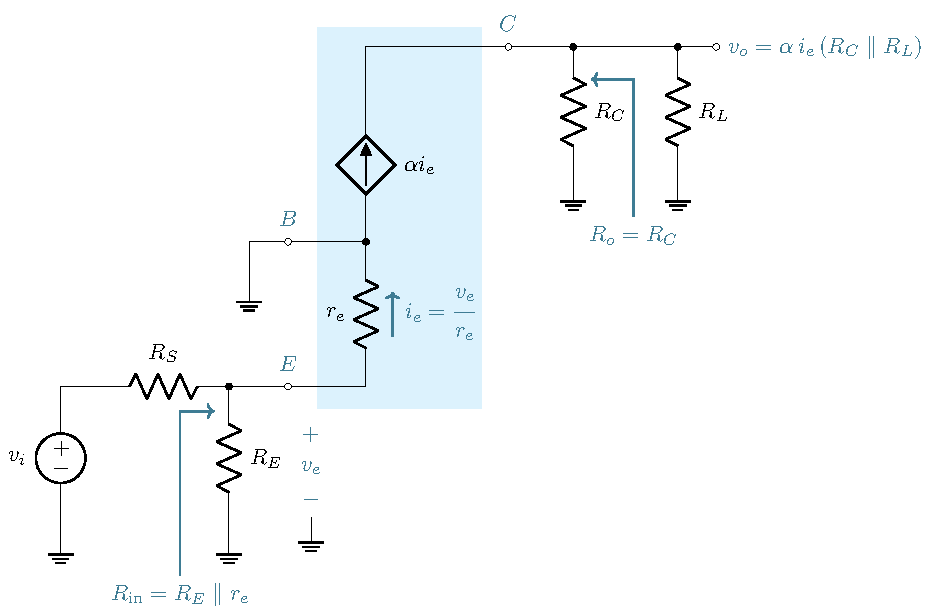
\includegraphics{figuras/fig_q2_T}
\caption{Circuito de sinal da Questão 2 com o transistor no modelo T, na região sombreada.}
\label{fig:q2-T}
\end{figure}

No emissor, $R_E$ e $r_e$ ficam em paralelo e formam um divisor com $R_S$; no coletor, a corrente $\alpha i_e = g_mv_e$ desce por $R_C\parallel R_L = 2{,}826\kohm$:
\begin{align*}
R_{\mathrm{in}} &= R_E\parallel r_e = 12{,}94\Om,\\[4pt]
\frac{v_e}{v_i} &= \frac{R_{\mathrm{in}}}{R_{\mathrm{in}}+R_S} = \frac{12{,}94}{1013} = 0{,}01277,\\[4pt]
\frac{v_o}{v_e} &= g_m(R_C\parallel R_L) = 216{,}0,\\[4pt]
\frac{v_o}{v_i} &= \frac{v_e}{v_i}\cdot\frac{v_o}{v_e} = 0{,}01277\times216{,}0 = 2{,}76.
\end{align*}

\resposta $v_o/v_i = +2{,}76$~V/V, ou 8,8~dB, sem inversão de fase. O ganho é pequeno porque a resistência de entrada do base-comum, 13~$\Omega$, é muito menor que $R_S = 1\kohm$, e 98,7\% de $v_i$ fica em $R_S$.

%-------------------------------------------------------------------
\section{Item (b): frequência de corte superior}
%-------------------------------------------------------------------

No modelo T, $C_\pi$ fica entre emissor e base e $C_\mu$ entre coletor e base (Figura~\ref{fig:q2-hf}). Com a base em terra, $C_\pi$ liga o emissor ao terra e $C_\mu$ liga o coletor ao terra. Nenhuma capacitância liga a entrada à saída, então nenhuma é multiplicada pelo ganho como prevê o teorema de Miller, e por isso o base-comum tem banda larga. O método das constantes de tempo de circuito aberto estima $f_H\approx1/(2\pi\sum R_iC_i)$, com $v_i = 0$:
\begin{gather*}
R_\pi = R_S\parallel R_E\parallel r_e = 12{,}77\Om,\qquad \tau_\pi = 10\un{pF}\times12{,}77\Om = 0{,}1277\un{ns},\\[2pt]
R_\mu = R_C\parallel R_L = 2{,}826\kohm,\qquad \tau_\mu = 1\un{pF}\times2826\Om = 2{,}826\un{ns},\\[2pt]
f_H\approx\frac{1}{2\pi(\tau_\pi+\tau_\mu)} = \frac{1}{2\pi\times2{,}954\un{ns}} = 53{,}9\un{MHz}.
\end{gather*}
Olhando para o coletor, o transistor tem resistência infinita, porque $V_A = \infty$; por isso $R_\mu$ inclui só $R_C$ e $R_L$.

\begin{figure}[htbp]
\centering
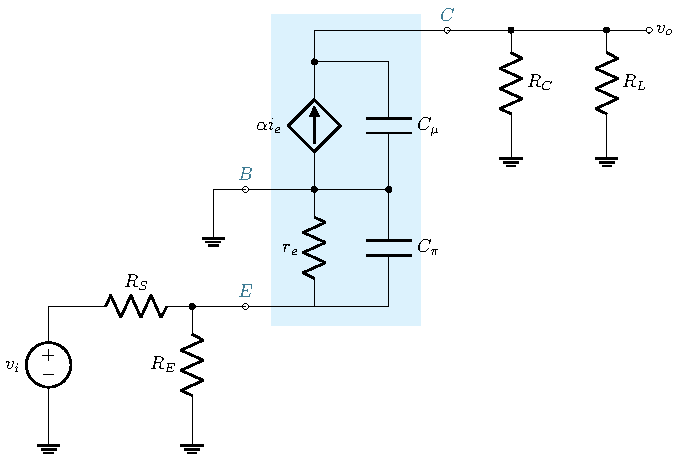
\includegraphics{figuras/fig_q2_hf}
\caption{Circuito de sinal da Questão 2 em altas frequências, com $C_\pi$ e $C_\mu$ no modelo T.}
\label{fig:q2-hf}
\end{figure}

Aqui o valor exato também pode ser calculado. Os nós do emissor e do coletor só se ligam pela fonte controlada, que leva sinal num sentido só; cada capacitor produz um polo separado, em $f_\pi = 1/(2\pi\tau_\pi) = 1{,}246$~GHz e $f_\mu = 1/(2\pi\tau_\mu) = 56{,}32$~MHz. Igualando o ganho relativo a $1/\sqrt2$, com $x = f^2$, $a = f_\mu^2$ e $b = f_\pi^2$:
\begin{equation*}
\left[1+\frac{x}{a}\right]\left[1+\frac{x}{b}\right] = 2
\;\Rightarrow\;
x^2 + (a+b)\,x - ab = 0
\;\Rightarrow\;
x = 3159\un{MHz^2},\qquad f_H = 56{,}2\un{MHz}.
\end{equation*}

\resposta $f_H = 53{,}9$~MHz pelo método das constantes de tempo de circuito aberto; o valor exato é 56,2~MHz, fixado por $C_\mu$ e $R_C\parallel R_L$. O método fica um pouco abaixo do valor exato, do lado seguro.

%-------------------------------------------------------------------
\section{Item (c): projeto dos capacitores de acoplamento}
%-------------------------------------------------------------------

Usa-se o mesmo método da Questão 1(c), agora para $f_L = 20$~Hz. Com $v_i = 0$, $C_{C1}$ vê $R_S$ em série com a entrada do emissor, $R_E\parallel r_e$; $C_{C2}$ vê $R_C$ em série com $R_L$, porque o coletor tem resistência infinita. Como o estágio é unilateral, uma resistência não depende do outro capacitor. $C_{C1}$, que vê a menor resistência, recebe 90\% de $f_L$ (Tabela~\ref{tab:q2-cap}).

\begin{table}[H]
\centering
\caption{Resistência vista por cada capacitor de acoplamento da Questão 2 e capacitores do método.}
\label{tab:q2-cap}
\begin{tabular}{lcccc}
\toprule
Capacitor & Resistência vista & Valor & $f_{Pi}$ & $C_i = 1/(2\pi R_if_{Pi})$ \\
\midrule
$C_{C1}$ & $R_S + (R_E\parallel r_e)$ & 1012,9~$\Omega$ & 18~Hz & 8,729~\textmu F \\
$C_{C2}$ & $R_C + R_L$ & 11,5~k$\Omega$ & 2~Hz & 6,920~\textmu F \\
\bottomrule
\end{tabular}
\end{table}

Os dois filtros são independentes, então o $f_L$ real sai do produto dos dois fatores $f/\sqrt{f^2+f_{Pi}^2}$ igualado a $1/\sqrt2$, uma equação do segundo grau em $f^2$:
\begin{equation*}
f^4 - (f_{P1}^2+f_{P2}^2)\,f^2 - f_{P1}^2f_{P2}^2 = 0
\;\Rightarrow\;
f_L^2 = \frac{328+\sqrt{328^2+4\times1296}}{2} = 331{,}9
\;\Rightarrow\;
f_L = 18{,}22\un{Hz}.
\end{equation*}
Multiplicar os dois capacitores por $18{,}22/20 = 0{,}911$ leva $f_L$ a 20~Hz: $C_{C1} = 7{,}95$~\textmu F e $C_{C2} = 6{,}30$~\textmu F.

\resposta $C_{C1} = 7{,}95$~\textmu F e $C_{C2} = 6{,}30$~\textmu F dão $f_L = 20$~Hz. Os valores diretos do método, 8,73~\textmu F e 6,92~\textmu F, dão 18,2~Hz.

%-------------------------------------------------------------------
\section{Item (d): simulações e comparação}
%-------------------------------------------------------------------

Os arquivos são \texttt{q2\_cc.cir}, \texttt{q2\_transiente.cir} e \texttt{q2\_frequencia.cir}; o último simula os dois conjuntos de capacitores. O transistor é um PNP com $\texttt{BF} = 100$, $V_A$ infinito e capacitâncias internas nulas, que são os padrões do LTspice; $C_\pi$ e $C_\mu$ entram como capacitores externos. A corrente de saturação foi ajustada para $\texttt{IS} = 3{,}37$~fA, para que $V_{EB}$ seja 0,70~V na corrente de polarização, como pede o enunciado; com o padrão, $10^{-16}$ A, daria 0,79~V. O transiente usa 10~mV de pico em 10~kHz. A Tabela~\ref{tab:q2-sim} compara os resultados, e as Figuras~\ref{fig:q2-sim-tran} e~\ref{fig:q2-sim-freq} mostram as curvas.

\begin{table}[H]
\centering
\caption{Questão 2: valores calculados nos itens (a) a (c) e simulados.}
\label{tab:q2-sim}
\begin{tabular}{lccc}
\toprule
Grandeza & Calculado & Simulado & Erro \\
\midrule
$I_E$ & 1,930~mA & 1,930~mA & $0{,}00\%$ \\
$I_C$ & 1,911~mA & 1,911~mA & $0{,}00\%$ \\
$V_C$ & $-12{,}58$~V & $-12{,}58$~V & $0{,}00\%$ \\
$V_{EC}$ & 13,28~V & 13,28~V & $0{,}00\%$ \\
$v_o/v_i$, transiente em 10~kHz & 2,759 & 2,758 & $-0{,}04\%$ \\
$v_o/v_i$, resposta em frequência em 10~kHz & 2,759 & 2,757 & $-0{,}05\%$ \\
$f_H$, método das constantes de tempo & 53,88~MHz & 56,19~MHz & $+4{,}29\%$ \\
$f_H$, valor exato & 56,20~MHz & 56,19~MHz & $-0{,}01\%$ \\
$f_L$, capacitores do método & 18,22~Hz & 18,21~Hz & $-0{,}05\%$ \\
$f_L$, capacitores ajustados & 20,00~Hz & 20,00~Hz & $-0{,}02\%$ \\
\bottomrule
\end{tabular}
\end{table}

A polarização coincide porque $I_S$ foi escolhida para dar $V_{EB} = 0{,}7$~V. O simulador usa $V_T = kT/q = 25{,}86$~mV, a 27 $^\circ$C, e não 25~mV; $r_e$ passa de 12,95~$\Omega$ para 13,40~$\Omega$, mas $R_S$ domina o divisor de entrada e o ganho muda só 0,05\%. A fase em 10~kHz é $+0{,}1^\circ$. O $f_H$ simulado confirma o valor exato do item (b), e a estimativa pelas constantes de tempo fica 4\% abaixo, como se espera do método. Os dois $f_L$ simulados confirmam o item (c), inclusive o ajuste para 20~Hz.

\begin{figure}[htbp]
\centering
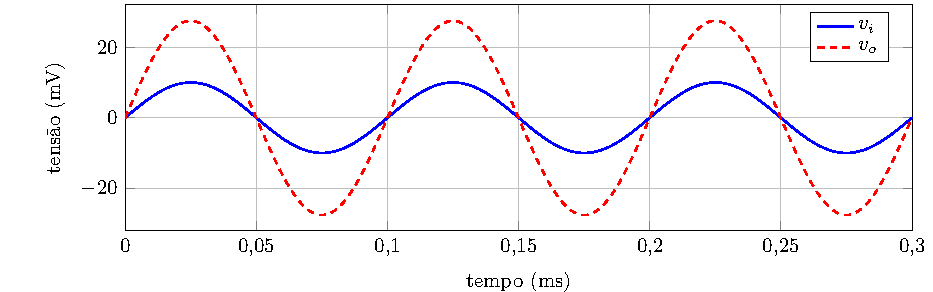
\includegraphics{figuras/fig_c_q2_transiente}
\caption[Questão 2: entrada e saída simuladas no transiente.]{Questão 2: entrada e saída simuladas no transiente, com 10~mV de pico em 10~kHz. A saída está em fase com a entrada.}
\label{fig:q2-sim-tran}
\end{figure}

\begin{figure}[htbp]
\centering
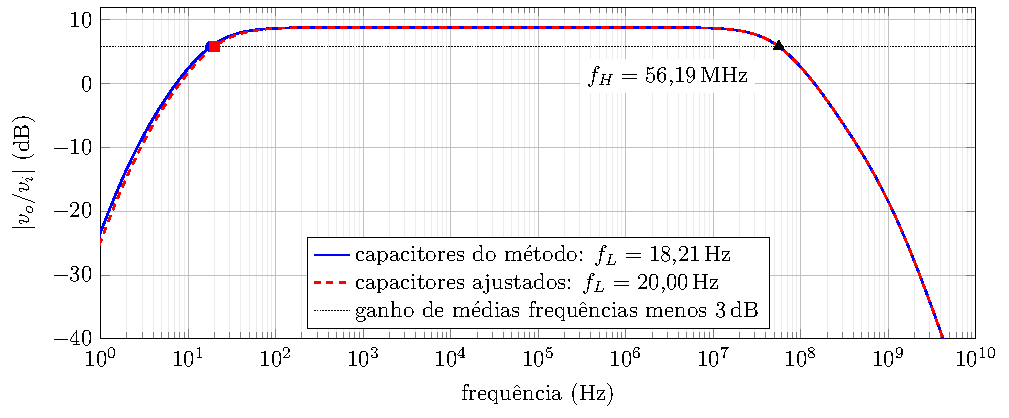
\includegraphics[width=\textwidth]{figuras/fig_c_q2_frequencia}
\caption[Questão 2: módulo do ganho simulado em função da frequência.]{Questão 2: módulo do ganho simulado em função da frequência, com os capacitores do método (8,73~\textmu F e 6,92~\textmu F) e com os ajustados (7,95~\textmu F e 6,30~\textmu F). O círculo e o quadrado marcam $f_L$ de cada conjunto, e o triângulo, $f_H$, onde as curvas cruzam a linha 3~dB abaixo do ganho de médias frequências.}
\label{fig:q2-sim-freq}
\end{figure}

%===================================================================
\chapter{Questão 3}
%===================================================================

A Questão 3 trata do amplificador diferencial com MOSFETs da Figura~\ref{fig:q3-circuito}. Os dois transistores são idênticos, com
\begin{equation*}
k_n'\frac{W}{L} = 100\un{\mu A/V^2}, \qquad \lambda = 0{,}02\un{V^{-1}}, \qquad V_{tn} = 1\un{V}.
\end{equation*}

\begin{figure}[htbp]
\centering
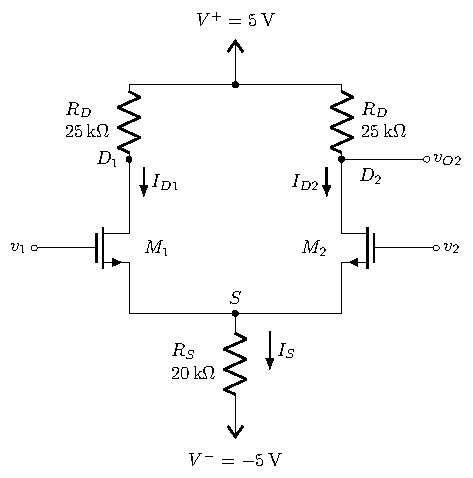
\includegraphics{figuras/fig_q3_circuito}
\caption{Amplificador diferencial com MOSFETs da Questão 3.}
\label{fig:q3-circuito}
\end{figure}

É um \textbf{par diferencial}: dois transistores iguais com as fontes ligadas juntas e alimentadas por $R_S$, que faz o papel da fonte de corrente de polarização. A saída é tomada só no dreno de M2, em relação ao terra.

%-------------------------------------------------------------------
\section{Item (a): \texorpdfstring{$I_S$, $I_{D1}$, $I_{D2}$ e $v_{O2}$ para $v_1 = v_2 = 0$}{IS, ID1, ID2 e vO2 para v1 = v2 = 0}}
%-------------------------------------------------------------------

Com as duas portas em 0~V, o circuito é simétrico (Figura~\ref{fig:q3-cc}): $I_{D1} = I_{D2} = I_D$, $I_S = 2I_D$ e o nó das fontes fica em $V_S = -V_{GS}$. A corrente em $R_S$ é a soma das duas correntes de dreno; com $V_{GS} = 1 + V_{OV}$,
\begin{equation*}
I_S = \frac{5 - V_{GS}}{20\kohm} = 2\times\frac12\times100\un{\mu A/V^2}\times V_{OV}^2
\;\Rightarrow\; 4 - V_{OV} = 2\,V_{OV}^2
\;\Rightarrow\; V_{OV} = \frac{-1\pm\sqrt{33}}{4}.
\end{equation*}
A raiz negativa, $-1{,}686$~V, é descartada. Ficam $V_{OV} = 1{,}186$~V, $V_{GS} = 2{,}186$~V e
\begin{gather*}
I_S = \frac{5 - 2{,}186}{20\kohm} = 140{,}7\uA,\qquad I_{D1} = I_{D2} = \frac{I_S}{2} = 70{,}35\uA,\\[2pt]
v_{O2} = 5 - 25\kohm\times70{,}35\uA = 3{,}241\un{V}.
\end{gather*}
Com $V_{DS} = 3{,}241 - (-2{,}186) = 5{,}427$~V $\geq V_{OV}$, os dois transistores estão saturados (Tabela~\ref{tab:q3-cc}).

\begin{figure}[htbp]
\centering
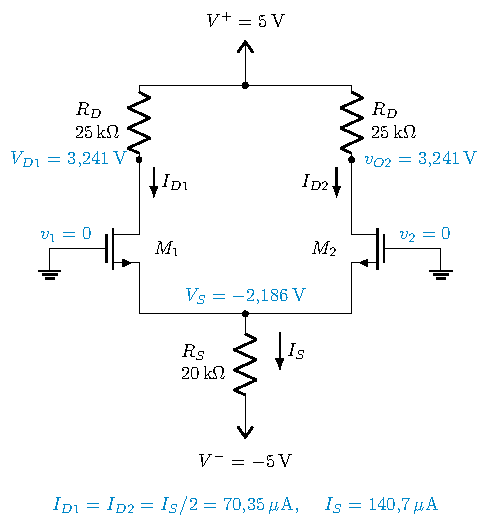
\includegraphics{figuras/fig_q3_cc}
\caption{Circuito c.c. da Questão 3 com $v_1 = v_2 = 0$ e os valores calculados.}
\label{fig:q3-cc}
\end{figure}

\begin{table}[H]
\centering
\caption{Polarização dos transistores da Questão 3 e verificação da saturação.}
\label{tab:q3-cc}
\begin{tabular}{lcccccc}
\toprule
 & $I_D$ & $V_{GS}$ & $V_{OV}$ & $V_{DS}$ & $V_{GS}>V_{tn}$? & $V_{DS}\geq V_{OV}$? \\
\midrule
M1 e M2 & 70,35~\textmu A & 2,186~V & 1,186~V & 5,427~V & Sim & Sim (folga de 4,2~V) \\
\bottomrule
\end{tabular}
\end{table}

\resposta $I_S = 140{,}7$~\textmu A, $I_{D1} = I_{D2} = 70{,}35$~\textmu A e $v_{O2} = 3{,}241$~V.

%-------------------------------------------------------------------
\section{Item (b): ganho diferencial, ganho em modo comum e \texorpdfstring{CMRR$_{dB}$}{CMRR}}
%-------------------------------------------------------------------

Os parâmetros de sinal são
\begin{equation*}
g_m = \frac{2\times70{,}35\uA}{1{,}186\un{V}} = 118{,}6\uAV,\qquad r_o = \frac{1}{0{,}02\times70{,}35\uA} = 710{,}8\kohm.
\end{equation*}
As entradas se escrevem como $v_1 = v_{icm} + v_{id}/2$ e $v_2 = v_{icm} - v_{id}/2$, com $v_{id} = v_1 - v_2$ e $v_{icm} = (v_1+v_2)/2$. Por superposição, $v_{o2} = A_dv_{id} + A_{cm}v_{icm}$. O circuito é simétrico e, para o sinal, linear; por isso cada parcela pode ser obtida de metade do circuito, a de M2 \cite{sedra,notas}.

\subsection{Ganho diferencial}

Com $v_1 = +v_{id}/2$ e $v_2 = -v_{id}/2$ (Figura~\ref{fig:q3-dif}), a excitação é antissimétrica e a resposta também. O nó das fontes está sobre o eixo de simetria, então sua tensão de sinal satisfaz $v_s = -v_s$, isto é, $v_s = 0$: é um terra virtual, mesmo com $r_o$. A corrente de sinal em $R_S$ é nula, e $R_S$ não afeta $A_d$.

\begin{figure}[htbp]
\centering
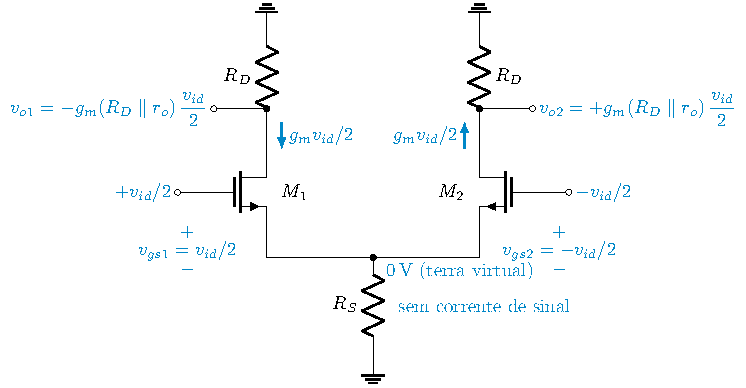
\includegraphics{figuras/fig_q3_dif}
\caption{Par diferencial da Questão 3 com entrada diferencial e as fontes c.c. em terra.}
\label{fig:q3-dif}
\end{figure}

O lado de M2 vira um amplificador fonte-comum com a porta em $-v_{id}/2$ e a fonte em terra (Figura~\ref{fig:q3-dif-meio}). No dreno, $R_D$ e $r_o$ ficam em paralelo:
\begin{gather*}
v_{o2} = -g_m\left(-\frac{v_{id}}{2}\right)(R_D\parallel r_o)
\;\Rightarrow\;
A_d = \frac{v_{o2}}{v_{id}} = \frac{1}{2}g_m(R_D\parallel r_o),\\[2pt]
\boxed{A_d = 0{,}5\times0{,}1186\mAV\times24{,}15\kohm = 1{,}432}
\end{gather*}
O ganho é positivo: quando $v_1$ sobe em relação a $v_2$, a corrente de M2 cai e $v_{o2}$ sobe. O fator $1/2$ vem da entrada, porque a porta de M2 recebe só $v_{id}/2$; com saída diferencial, $v_{o2} - v_{o1}$, o ganho seria o dobro, 2,865.

\begin{figure}[htbp]
\centering
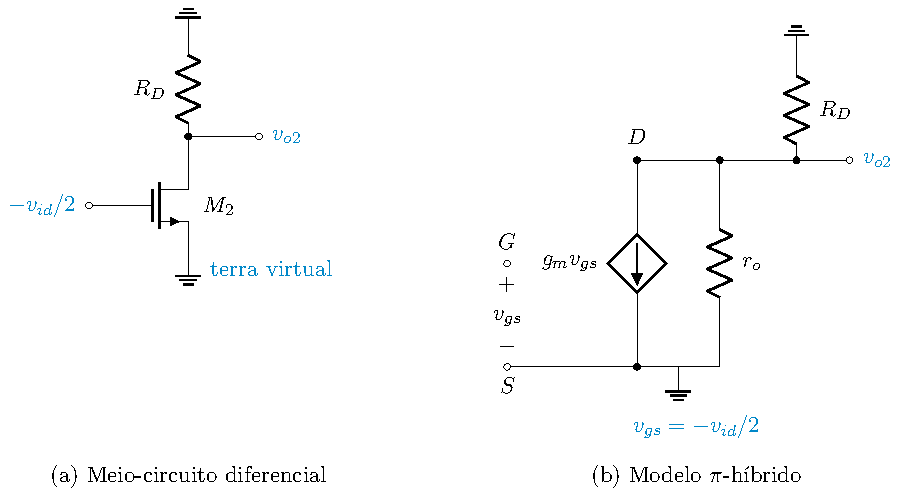
\includegraphics{figuras/fig_q3_dif_meio}
\caption{Meio-circuito diferencial de M2 e seu modelo $\pi$-híbrido com $r_o$.}
\label{fig:q3-dif-meio}
\end{figure}

\subsection{Ganho em modo comum}

Com $v_1 = v_2 = v_{icm}$, os dois lados conduzem a mesma corrente de sinal $i_d$ e por $R_S$ passa $2i_d$: o nó das fontes acompanha a entrada, com $v_s = 2R_Si_d$. A mesma tensão apareceria se cada transistor tivesse sua própria resistência $2R_S$, pois $R_S = 2R_S\parallel2R_S$; o fio entre as duas metades não conduz corrente e pode ser cortado. Fica o meio-circuito da Figura~\ref{fig:q3-cm-meio}, cujas equações são
\begin{gather*}
v_{gs} = v_{icm} - v_s, \qquad v_s = 2R_S\,i_d,\\[4pt]
v_{o2} = -R_D\,i_d, \qquad i_d = g_mv_{gs} + \frac{v_{o2}-v_s}{r_o}.
\end{gather*}

\begin{figure}[htbp]
\centering
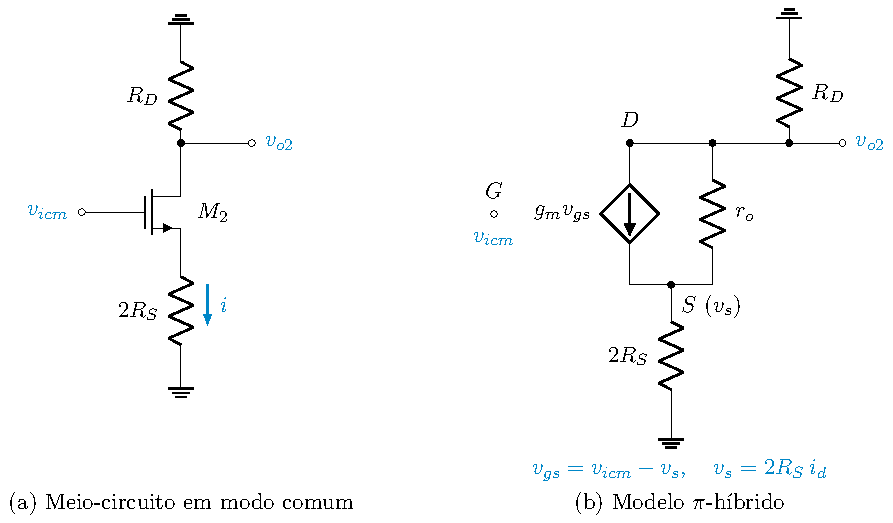
\includegraphics{figuras/fig_q3_cm_meio}
\caption[Meio-circuito em modo comum de M2 e seu modelo $\pi$-híbrido com $r_o$.]{Meio-circuito em modo comum de M2, com $R_S$ representado por $2R_S$, e seu modelo $\pi$-híbrido com $r_o$.}
\label{fig:q3-cm-meio}
\end{figure}

Substituindo as três primeiras na quarta, obtém-se $i_d\left[1 + 2g_mR_S + (R_D+2R_S)/r_o\right] = g_mv_{icm}$; com $v_{o2} = -R_Di_d$,
\begin{gather*}
A_{cm} = \frac{v_{o2}}{v_{icm}} = \frac{-g_mR_D}{1 + 2g_mR_S + (R_D+2R_S)/r_o},\\[6pt]
\boxed{A_{cm} = \frac{-2{,}965}{1 + 4{,}745 + 0{,}091} = -0{,}508}
\end{gather*}
A aproximação $A_{cm}\approx-R_D/(2R_S) = -0{,}625$ não vale aqui, porque supõe $2g_mR_S\gg1$, e $2g_mR_S = 4{,}7$.

\subsection{Rejeição em modo comum}

A taxa de rejeição em modo comum compara os dois ganhos:
\begin{equation*}
\text{CMRR} = \left|\frac{A_d}{A_{cm}}\right| = \frac{1{,}432}{0{,}508} = 2{,}819,
\qquad
\text{CMRR}_{dB} = 20\log_{10}2{,}819 = 9{,}00\un{dB}.
\end{equation*}
Sem $r_o$, os resultados seriam $A_d = 1{,}483$, $A_{cm} = -0{,}516$ e $\text{CMRR}_{dB} = 9{,}16$~dB: $r_o$ pesa pouco, porque é muito maior que $R_D$.

\resposta $A_d = +1{,}432$~V/V, $A_{cm} = -0{,}508$~V/V e $\text{CMRR}_{dB} = 9{,}00$~dB. A rejeição é baixa porque a saída é tomada de um lado só e porque $R_S = 20\kohm$ é uma fonte de corrente pobre; com resistência de cauda infinita, $A_{cm}$ seria zero.

%-------------------------------------------------------------------
\section{Item (c): simulações e comparação}
%-------------------------------------------------------------------

Os arquivos são \texttt{q3\_cc.cir}, com $v_1 = v_2 = 0$; \texttt{q3\_transiente\_diferencial.cir}, com $v_{id} = 10$~mV de pico em 1~kHz e $v_{icm} = 0$; e \texttt{q3\_transiente\_modo\_comum.cir}, com $v_{icm} = 10$~mV de pico em 1~kHz e $v_{id} = 0$. Duas fontes controladas fazem $v_1 = v_{icm} + v_{id}/2$ e $v_2 = v_{icm} - v_{id}/2$; se o sinal fosse aplicado só em $v_1$, a entrada teria também $v_{icm} = v_1/2$, e a saída mediria $A_d + A_{cm}/2 = 1{,}178$, e não $A_d$. O MOSFET é o nível 1 do LTspice com $\texttt{KP} = 100\un{\mu A/V^2}$, $W = L$, $\texttt{VTO} = 1$~V e $\texttt{LAMBDA} = 0{,}02$/V. A Tabela~\ref{tab:q3-sim} compara os resultados.

\begin{table}[H]
\centering
\caption{Questão 3: valores calculados nos itens (a) e (b) e simulados.}
\label{tab:q3-sim}
\begin{tabular}{lccc}
\toprule
Grandeza & Calculado & Simulado & Erro \\
\midrule
$I_S$ & 140,7~\textmu A & 143,1~\textmu A & $+1{,}74\%$ \\
$I_{D1} = I_{D2}$ & 70,35~\textmu A & 71,57~\textmu A & $+1{,}74\%$ \\
$v_{O2}$ & 3,241~V & 3,211~V & $-0{,}94\%$ \\
$A_d$ & $+1{,}432$ & $+1{,}524$ & $+6{,}42\%$ \\
$A_{cm}$ & $-0{,}508$ & $-0{,}514$ & $+1{,}21\%$ \\
$\text{CMRR}_{dB}$ & 9,00~dB & 9,44~dB & $+4{,}84\%$ \\
\bottomrule
\end{tabular}
\end{table}

Os ganhos foram medidos nos transientes da Figura~\ref{fig:q3-sim}. Com $v_{id} = 10$~mV de pico, $v_{o2}$ varia $\pm15{,}24$~mV em torno de 3,211~V, em fase com $v_{id}$, o que dá $A_d = +1{,}524$. Com $v_{icm} = 10$~mV de pico, $v_{o2}$ varia $\pm5{,}14$~mV em oposição de fase, o que dá $A_{cm} = -0{,}514$. A rejeição simulada é $1{,}524/0{,}514 = 2{,}964$, ou 9,44~dB.

\begin{figure}[htbp]
\centering
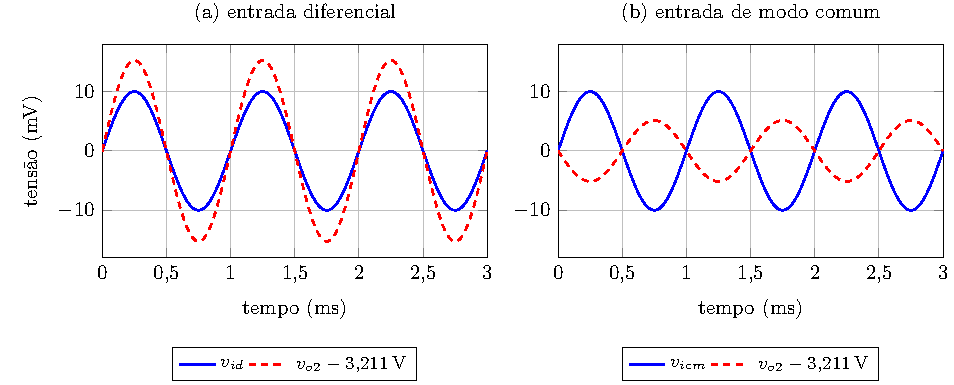
\includegraphics{figuras/fig_c_q3_transientes}
\caption[Questão 3: transientes simulados com entrada diferencial e em modo comum.]{Questão 3: transientes simulados com entrada diferencial (a) e em modo comum (b). A saída aparece como variação em torno do valor de repouso $v_{O2} = 3{,}211$~V.}
\label{fig:q3-sim}
\end{figure}

Como na Questão 1, a diferença vem do fator $(1+\lambda V_{DS})$, que o simulador mantém na polarização. Aqui ele pesa mais, porque $\lambda = 0{,}02$/V e $V_{DS}\approx5{,}3$~V: o fator vale 1,107. Resolvendo o item (a) com ele, obtêm-se $V_{GS} = 2{,}137$~V, $I_D = 71{,}57$~\textmu A e $v_{O2} = 3{,}211$~V, os valores simulados. Com $V_{OV} = 1{,}137$~V, $g_m$ passa a 125,9~\textmu A/V e $r_o = (1+\lambda V_{DS})/(\lambda I_D)$ a 773~k$\Omega$; levados às fórmulas do item (b), dão $A_d = 1{,}524$, $A_{cm} = -0{,}514$ e $\text{CMRR}_{dB} = 9{,}44$~dB, iguais aos simulados.

%===================================================================
\chapter{Conclusão}
\label{cap:conclusao}
%===================================================================

A Tabela~\ref{tab:resumo} reúne as respostas. Na Questão 2 cálculo e simulação coincidem dentro de 0,05\%, exceto a estimativa de $f_H$ pelas constantes de tempo, 4\% abaixo do valor exato, como se espera do método. Nas Questões 1 e 3 o simulado fica até 6,4\% acima no ganho, porque a polarização calculada despreza o fator $(1+\lambda V_{DS})$; refazendo as contas com ele, os valores simulados se reproduzem. No projeto dos capacitores de acoplamento, a soma das frequências superestima $f_L$ quando nenhum capacitor domina, e os capacitores foram ajustados por um fator comum para atingir 100~Hz e 20~Hz.

\begin{table}[H]
\centering
\caption{Resumo das respostas calculadas e simuladas.}
\label{tab:resumo}
\setlength{\tabcolsep}{4pt}
\begin{tabular}{llccc}
\toprule
Item & Grandeza & Calculado & Simulado & Erro \\
\midrule
1(a) & $I_{D1}$ & 0,757~mA & 0,759~mA & $+0{,}3\%$ \\
 & $I_{D2}$ & 0,757~mA & 0,758~mA & $+0{,}2\%$ \\
 & $V_{DS1}$ & 12,43~V & 12,41~V & $-0{,}2\%$ \\
 & $V_{DS2}$ & 8,65~V & 8,63~V & $-0{,}3\%$ \\ \addlinespace
1(b) & $v_o/v_i$ & 2,40~V/V (7,6~dB) & 2,53~V/V (8,1~dB) & $+5{,}5\%$ \\ \addlinespace
1(c) & $f_L$ com 34,4~nF, 3,07~\textmu F e 2,00~\textmu F & 100~Hz & 99,98~Hz & $-0{,}02\%$ \\
\midrule
2(a) & $v_o/v_i$ & 2,76~V/V (8,8~dB) & 2,76~V/V (8,8~dB) & $-0{,}05\%$ \\ \addlinespace
2(b) & $f_H$ pelo método & 53,9~MHz & 56,2~MHz & $+4{,}3\%$ \\
 & $f_H$ exato & 56,2~MHz & 56,2~MHz & $-0{,}01\%$ \\ \addlinespace
2(c) & $f_L$ com 7,95~\textmu F e 6,30~\textmu F & 20~Hz & 20,00~Hz & $-0{,}02\%$ \\
\midrule
3(a) & $I_S$ & 140,7~\textmu A & 143,1~\textmu A & $+1{,}7\%$ \\
 & $I_{D1} = I_{D2}$ & 70,35~\textmu A & 71,57~\textmu A & $+1{,}7\%$ \\
 & $v_{O2}$ & 3,241~V & 3,211~V & $-0{,}9\%$ \\ \addlinespace
3(b) & $A_d$ & 1,432 & 1,524 & $+6{,}4\%$ \\
 & $A_{cm}$ & $-0{,}508$ & $-0{,}514$ & $+1{,}2\%$ \\
 & $\text{CMRR}_{dB}$ & 9,00~dB & 9,44~dB & $+4{,}8\%$ \\
\bottomrule
\end{tabular}
\end{table}

%===================================================================
\clearpage
\phantomsection
\addcontentsline{toc}{chapter}{Referências Bibliográficas}
\begin{thebibliography}{9}
\bibitem{sedra} A. S. Sedra, K. C. Smith, T. C. Carusone e V. Gaudet, \textit{Circuitos Microeletrônicos}, 8. ed. Rio de Janeiro: LTC, 2023.
\bibitem{notas} M. Lima, \textit{Eletrônica Analógica II: notas de aula}. Faculdade de Engenharia, Universidade Federal de Juiz de Fora.
\end{thebibliography}

\section*{Declaração de uso de inteligência artificial}
\addcontentsline{toc}{chapter}{Declaração de uso de inteligência artificial}

Planejamos e conduzimos a atividade do começo ao fim: fizemos todos os cálculos à mão, cada um com sua forma de resolver, e conferimos os resultados entre nós; Chrysthofer escreveu no Overleaf um rascunho com os gráficos, os arquivos de simulação, parte da teoria, as respostas e o método de resolução, e Angelo usou esse rascunho como base para o trabalho final. Usamos o assistente Claude, da Anthropic, como ferramenta de apoio no trabalho repetitivo: na fase do rascunho, montou com Chrysthofer o arquivo \LaTeX, as \textit{netlists} do LTspice, as curvas exportadas para os gráficos e os recortes dos circuitos do enunciado; na revisão final, conferiu as contas e as simulações e enxugou o texto para a entrega, o que revisamos e validamos com os cálculos que fizemos à mão. Também refez os gráficos a partir dos dados das simulações, redesenhou os esquemáticos para dar folga aos rótulos e conferiu a notação com os slides da disciplina.

\end{document}
